\newcommand{\be}{\mathbf{e}}
\newcommand{\bn}{\mathbf{n}}
\newcommand{\bx}{\mathbf{x}}

\section{Metrics}
\label{sec:metrics}
To measure the difference between depth images, we consider several metrics distinct from MSE used in most previous works. 
Our overall approach is to reduce the comparison of depth images to comparison of regular images generated from these depth fields, using various types of standard and perception-based metrics.

\paragraph{From depth maps to images.}  To approximate the appearance of a 3D model, we use  simple diffuse lighting, with directional light sources 
having light source directions $\bm{e}_i$. We do not take visibility into account. We use a camera corresponding to the acquisition point of view. For this simple model, the intensity $I_i$ at a point $(x,y)$ of the depth map is proportional to $\bm{e}_i \cdot \bm{n}(x,y)$, where $\bm{n}(x, y)$ is the value of 3D surface normals that get projected to point $(x,y)$ on the image. If we pick three orthogonal light directions $\bm{e}_1, \bm{e}_3, \bm{e}_3$ and concatenate the result, we obtain three components of the normal vector in the coordinate system defined by $\bm{e}_i$, see Figure~\ref{fig:normals_directions}. Images for any other lighting direction can be obtained as linear combinations of these three images. 

\begin{figure}[t]
\begin{center}
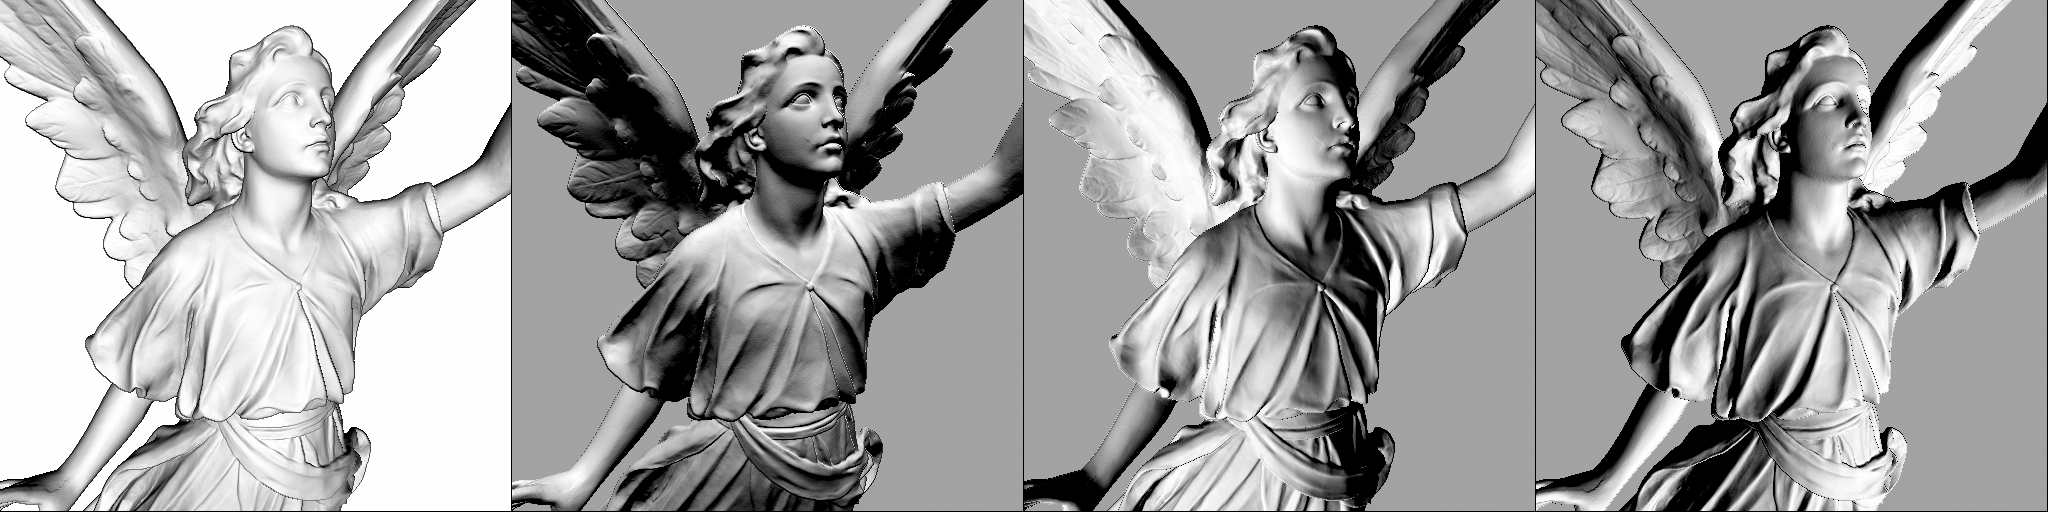
\includegraphics[width=0.95\columnwidth]{Figures/depth_superresolution/renderings.lucy.png}
\end{center}
   \caption{Renderings of surface used in our evaluation of the perceptually-based metrics.
   }
\label{fig:normals_directions}
\end{figure}

This suggests that the \emph{normal image} for the depth map can be viewed as a proxy for the space of possible images generated from the 3D geometry specified by this depth map in this simple model.  The normal for a depth map is estimated using standard finite differences.

\paragraph{Low-level error metrics.}  
%Given two depth maps $d_1$ and $d_2$ (\eg, the ground-truth high-resolution depth map and a map obtained by upsampling a low-resolution depth map), a metric computes a value capturing the difference between the two. 
The simplest difference between depth maps $d_1$ and $d_2$ based on visual difference is computed simply as either MSE or absolute value error between the normal images:
%\LA{Add sin2 formula that we use}
\begin{align*}
&\mathcal{E}_{\mathrm{RMSE}}(d_1,d_2) = \sqrt{\frac{1}{N}\sum_{i,j} \| n_{ij}^1- n_{ij}^2\|^2_2},\; \\
&\mathcal{E}_{\mathrm{ABS}}(d_1,d_2) = \frac{1}{N}\sum_{i,j} \| n_{ij}^1- n_{ij}^2\|_1.
\end{align*}  
There are a few closely related metrics, in particular, threshold-based ones, such as BadPix \cite{honauer2015hci}.
In our experiments we use another surface-aware error metric, closely related to \(\mathcal{E}_{\mathrm{RMSE}}\), which leads to faster convergence:
\[
\mathcal{E}_{\mathrm{SURF}}(d_1,d_2) = 1 - \left(\bm{n}^{1}\cdot \bm{n}^{2}\right)^2.
\]

Another set of measures introduced in \cite{honauer2015hci} are heuristic measures 
of various aspects of surface perception: foreground flattening/thinning, fuzziness, 
bumpiness, etc.  Most of them require a very specific segmentation of the image: detection of flat areas and depth discontinuities, which is difficult to do in general case, even for noise-free ground-truth images. 

%\LA{DZ: geometry-aware metrics from HCI stereo metrics paper (bumpiness etc.)?}
%\LA{DZ: maybe rename this to 'low-level geometric measures'?}

%\cite{honauer2015hci}
%\cite{honauer2016dataset}
%\cite{4dlightfieldbenchmark}

\paragraph{Perceptually-based metrics.}  We use two most common perceptually-based types of metrics: a statistics-based SSIM,  and several metrics based on measuring RMS distances between features in a trained neural net.   

\noindent\emph{SSIM \cite{wang2004image}.}  SSIM (structural similarity index measure) is a widely used metric 
that aims to take into account changes in local structure of an image, captured by a number of statistical quantities 
computed on a small window around each pixel. A per-pixel SSIM index is computed,  and the mean of per-pixel indices 
yields a global metric. For each pixel, 3 terms (the luminance term $\ell$, the contrast term $c$ and the structural term $s$, each normalized to be bounded by 1) 
are multiplied.  These terms are computed from the local means 
$\mu_x,\mu_y$, standard deviations $\sigma_x,\sigma_y$ and cross-covariance $\sigma_{xy}$ of corresponding local windows in two images $x$ and $y$, 
\begin{equation*}
    l(x,y) = \frac{2\mu_x \mu_y}{\mu_x^2 + \mu_y^2},\;
    c(x,y) = \frac{2\sigma_x \sigma_y}{\sigma_x^2 + \sigma_y^2},\;
    s(x,y) = \frac{\sigma_{xy} \sigma_y}{\sigma_x\sigma_y}
\end{equation*}
with small (relative to range) constants added to each numerator and denominator to avoid undefined behavior  for zero means or standard deviations. The luminance and contrast differences are captured by comparing means and standard deviations, and structure similarity is measured by correlation of normalized values in the neighborhood. DSSIM is a rescaling of SSIM computed as $(1-SSIM)/2$.

% test
%For a gray-scale image, FSIM is given by the sum of
%the combined similarity measures at pixels, weighted by \emph{phase congruency}:
%\begin{equation*}
%\mathcal{E}_{\mathrm{FSIM}} = \frac{\sum_{i,j} S_L(i,j)PC_m(i,j)}{\sum_{i,j} PC_m(i,j)}
%\end{equation*}  
%where $PC$ is the maximal phase congruency at a pixel between two images, $S_L = S_{PC} S_{G}$ is the  product of %phase congruency and gradient similarity measures.
%Phase congruency, with values in the 0 to 1 range,  measures correlation between phases of Fourier components of the image at a pixel, which was demonstrated to be
%a good indicator of locally important geometric features in an image (e.g., edges). Its computation using multiscale Gabor filters is described in \cite{zhang2011fsim}.
%$S_{G}$ and $S_{PC}$ measures are computed in a similar way: for a quantity $X$, the similarity measure is defined as $2X_1 X_2/(X_1^2 + X_2^2)$, which has values in the range $-1\ldots 1$, with 1 corresponding to equal numbers.


%\noindent\emph{HDR-VDP-2.} The HDR-VDP metric  \cite{mantiuk2011hdr} is computed as a superposition of several relatively complex  operators. At the first stage,  a modulated transfer function is applied to the Fourier transform of the input image, to model light-scattering in the eyes. Components corresponding to different photo-receptors in the eyes (rodes and three types of cones) are weighted by corresponding photo-sensitivity ratios, and then a transfer function taking into account the luminance masking effect is applied to each per-pixel value. At the second stage, a multi-scale decomposition of the  resulting signal is constructed using the steerable pyramid \cite{simoncelli1995steerable} is constructed. For all components of the decomposition  parametrized by the scale $f$ and orientation $o$, a noise-normalized difference $D[f,o](i,j)$, viewed as difference of corresponding steerable pyramid basis functions scaled by the difference of coefficients for $d^1$ and $d^2$,  is computed. The HDR-VDP-2 error measure is computed by a final weighted pooling step:

%\begin{equation*}
%\scriptsize
%\mathcal{E}_{\mathrm{VH2}} = \frac{1}{N_F N_O} \sum_f \sum_o w_f \log \left(\frac{1}{N} \sum_{i,j} D^2[f,o](i,j)  \right)
%\end{equation*}
%where the weights were optimized to match the experimental data in the best way. 
%\cite{wang2004image}
%\cite{wang2003multiscale}


\noindent\emph{Neural net-based metrics.} The overall underlying idea of all of these metrics is to compute an $L^2$ distance between features extracted
from a neural network.  Specifically, features $\bx_\ell$, $\ell = 1\ldots L$,
are extracted from $L$ layers of the network (with different $L$ for each network type).  If $\ell$-th layer feature is of dimension $H_\ell \times W_\ell \times C_\ell$,
where $H_\ell$ and $W_\ell$ are spatial dimensions and $C_\ell$ is the number of channels, then, in the simplest case, the error is computed as

\begin{equation*}
\mathcal{E}_{\mathrm{NN}} = \sum_\ell \frac{1}{{H_\ell W_\ell}} \sum_{h,w} \| \widehat{\bx}^{\ell,1}_{hw} - \widehat{\bx}^{\ell,2}_{hw}\|^2_2,
\end{equation*}
where $\widehat{\bx}_{hw}^\ell$ denotes the unit normalization of feature vectors along the channel direction. 
We use \cite{Zhang_2018_CVPR} choice of networks:  Alexnet \cite{krizhevsky2012imagenet} with, VGG  \cite{Simonyan14c} (5 layers are used from both),
and  Squezenet \cite{i2016squeezenet} (the first layer is used). 

%\DZ{ TODO We probably are not going to use all; eliminate the ones we do not; need to say what these are trained on}

